\documentclass[12pt]{article}

\usepackage[margin=1.0in]{geometry}
\usepackage{color}
\usepackage{times}
\usepackage[pdftex]{hyperref}
\usepackage{graphics}

\newcommand{\fillin}[1]{\textcolor{red}{\textsc{#1}}}

\pagestyle{empty}
\setlength{\parindent}{0in}
\setlength{\parskip}{2ex}
\renewcommand{\baselinestretch}{1.0}

\begin{document}

STAT 604: \hfill \fillin{Mu-Fen Hsieh}\\
Intro.\ to Statistical Computing \hfill \fillin{Sep. 4, 2006}

\begin{center}
\Large HW 1\\
\normalsize Due: September 5, 2006
\end{center}

Instructions:  The homework assignment editing this \LaTeX\ document.  Download the \LaTeX\ source from the class web page and study
it to learn more about \LaTeX.  Using VIM, replace the red text with appropriate information (leaving your answers wrapped in the
\texttt{$\backslash$fillin} command).  Run ``pdflatex'' on this document.

You will submit this assignment in two parts:
\begin{enumerate}
\item Print out the PDF file and bring it to class, and
\item Send an e-mail to:
\begin{center}
hw01@dahlgrapevine.org
\end{center}
\emph{before class} on the due date with two attachments:
\begin{itemize}
\item The \LaTeX\ source file, and
\item The generated PDF document.
\end{itemize}
Do not e-mail the assignment directly to the professor or grader.
\end{enumerate}

Please complete the following:
\begin{enumerate}
\item Subscribe to the class mailing list as described on the class webpage.
\item ``Paste'' a photograph of you below using a \LaTeX\ float.  Write your name in the caption and a sentence about something that makes you unique.  (See Tutorial XI in \href{http://www.stat.tamu.edu/~dahl/teaching/604/lecture/l02/ltxprimer.pdf}{\LaTeX\ Tutorials: A Primer}.)  If you do not have a photo, I can take one after class on Thursday.\\
\begin{figure}[h]
\centering
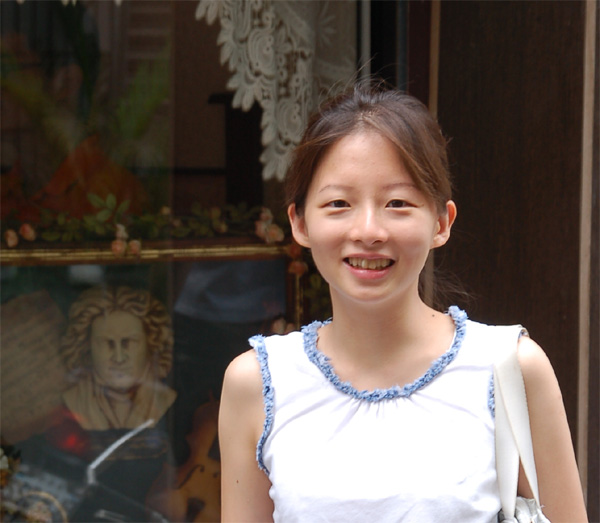
\includegraphics{mufen.jpg}
\caption{Mu-Fen Hsieh. One of her favorite poem is: ``
To see a world in a grain of sand 
and a heaven in a wild flower,
hold infinity in the palm of your hand
and eternity in an hour.''}
\end{figure}
\item What state or country are you from?  How is your name pronounced?\\
\fillin{I come from Taiwan. My name is pronounced \emph{M\`{u}f\={e}n X\`{i}e}}.
\item Is your ultimate intention to obtain a master's degree or a Ph.D.?\\
\fillin{I am a Ph.D.\ student.}
\item What was your major as an undergraduate?\\
\fillin{I majored in computer science as an undergraduate.}
\item How many statistics classes have you taken at the undergraduate level?  How many at the graduate level?\\
\fillin{I have taken ``Introduction to Probability \& Statistics'' at the undergraduate level and ``STAT 601 Statistical Analysis'' at the graduate level.}
\item Have you ever used Linux or UNIX before?  If so, describe the nature of your exposure.\\
\fillin{Yes. I started to use UNIX when I was a freshman in college. I used only email, telnet software and published static webpages on UNIX until I took the course ``UNIX System'' in my junior year. In the class, I learned the UNIX basics, and to code and compile programs on UNIX. I tried to install Redhat on my computer as well. After I graduated and went for a job, I also had a chance to administrate a Redhat system and to do a little shell programming and Make files.}
\item What programming languages, if any, have you been exposed to?  How many classes have you taken in each of these languages?  How many years experience do you have with each of them?\\
\fillin{I have learned Pascal in the course ``Introduction to Computer Science'' and ``Data Structures''; JAVA in ``The JAVA language''; Matlab in ``Numerical Methods'' and ``Neural Networks''; ASP and JavaScript in ``Web Programming''; C in ``Advanced Programming'', ``The C language'' and ``Windows Programming''; Perl in ``UNIX system''; and SQL in ``Introduction to Database System''. However, what I mostly used is the Java language, which I had 6-year experience.}
\item In late 1905, Albert Einstein published "Does the Inertia of a Body Depend Upon Its Energy Content?" which introduced the now famous equation that the energy of a body at rest (E) equals its mass (m) times the speed of light (c) squared.  Write this formula as a \LaTeX\ equation.\\
\fillin{\begin{equation}E = m \times c^{2}\end{equation}}
%This line and the next is "commented out".
\item Find a photograph on the Internet of a prominent statistician.  ``Paste'' the picture below using a \LaTeX\ float.  Write his/her name in the caption and a sentence about his/her notable contribution to statistics.  (Hint 1:  The \href{http://wikipedia.org}{Wikipedia} website is a great resource.  Hint 2:  See Tutorial XI in \href{http://www.stat.tamu.edu/~dahl/teaching/604/lecture/l02/ltxprimer.pdf}{\LaTeX\ Tutorials: A Primer}.)\\
\begin{figure}[h]
\centering
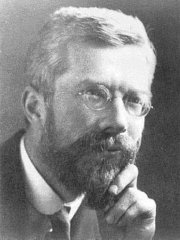
\includegraphics{RonaldFisher.jpg}
\caption{Sir Ronald Aylmer Fisher. He is a famous statistician who is known for maximum likelihood, Fisher information and analysis of variance. The historian of statistics Anders Hald said ``Fisher was a genius who almost single-handedly created the foundations for modern statistical science.''}
\end{figure}
\end{enumerate}
\end{document}
